%!TEX root=../document.tex

\section{Ergebnisse}
\label{sec:Ergebnisse}


\subsection{Nutzung von GPUs in normalen Desktop-Anwendungen}
\label{sec:Nutzung von GPUs in normalen Desktop-Anwendungen}
Im privaten Bereich gibt es praktisch keine Anwendung für GPGPU. Ausnahmen sind Programme für die Videobearbeitung. Typische Alltagssoftware lässt sich kaum parallelisieren. Im Bereich der Wissenschaft und Technik sieht es dann schon wieder anders aus. Hier machen mehrere GPGPU-taugliche Grafikkarten einen normalen PC zu einem Supercomputer.
Voraussetzung dafür ist ein hochleistungsfähiger Grafikprozessor, der bis zu 800 Kerne hat und parallel arbeitet. Damit ein Grafikprozessor überhaupt sinnvoll genutzt werden kann, muss die Anwendung eine sehr hohe Zahl von parallel ausführbaren Berechnungen enthalten. Wenn man die Rechenwerke eines Grafikprozessors kontinuierlich auslasten will, dann sollte man mindestens eine Millionen gleichartiger Berechnungen liefern können, sonst hat man gegenüber einer normalen CPU keine Vorteile. Die GPU-Rechenwerke müssen mit einem kontinuierlichen Datenstrom versorgt werden. Aus diesem Grund bezeichnet man sie auch als Stream-Prozessoren. \cite{elektronik_gpgpu}
Zu Ergänzen ist die erste Aussage auch noch mit Mathematikprogrammen wie Matlab oder ähnlichem.
\cite{matlab}

\subsubsection{Anwendungen}
\label{sec:Anwendungen}
\begin{itemize}
\item Physikalisch Simulationen (Strömung, Gravitation, Temperatur, Crash-Tests)
\item Komplexe Klimamodelle (Wettervorhersage)
\item Datenanalysen und Finanzmathematik
\item Verarbeitung von akustischen und elektrischen Signalen
\item CT- und Ultraschall-Bildrekonstruktion
\item Modellieren von Molekühlstrukturen
\item Kryptografie
\item Neuronale Netze
\item Videotranskodierung
\end{itemize}

\subsection{Vorteile der GPU bei rechenintensiven Anwendungen}
\label{sec:Vorteile der GPU bei rechenintensiven Anwendungen}
GPUs haben den Vorteil, dass sie auf spezielle Arten von Prozessen optimiert sind. CPUs sind hingegen darauf ausgelegt beliebige Aufgaben zu verarbeiten. Um rechenintensive Anwendungen auch tatsächlich auf der GPU laufen lassen zu können, müssen/sollten diese gut parallelisierbar sein. 
Im Vergleich zur CPU hat man wesentlich mehr Kerne auf die parallelisiert werden kann.

\subsection{Entwicklungsumgebungen und Programmiersprachen}
Von NVidia wird unter Anderem eine Visual Studio Abwandlung namens NSight zur Verfügung gestellt, welche es einem ermöglicht in CUDA C/C++, OpenCL, DirectCompute, Direct3D, and OpenGL zu programmieren.\\
OpenCL Studio eröffnet einem die Möglichkeit mit OpenCL und OpenGL zu arbeiten.\\
NVidia CUDA Toolkit bietet einem die Möglichkeit CUDA Applikationen in C und C++ zu Programmieren.
Applikationen für OpenCL werden zum Großteil in C oder C++ programmiert. OpenCL C/C++ bieten die Option direkt für OpenCL zu programmieren.
Bei der APP(Accelerated Parallel Processing) SDK von AMD, handelt es sich um eine Technologie, welche es einem ermöglicht die GPU neben dem Verarbeiten von Grafiken auch für weitere Dinge zu verwenden. Mit der APP-SDK kann unter anderem in Visual Studio programmiert werden. \cite{appsdk}\\
Bei C++ AMP (Accelerated Massive Parallelism) handelt es sich um ein Programmiermodell, welches die Programmiersprache C++  um eine Library und die Fähigkeit Code auf die GPU auszulagern erweitert.
Es setzt auf DirectX 11 auf. \cite{AMP}
\subsection{Transkompilieren}
Um bestehende Applikationen auf GPUs sinnvoll zu nutzen, müssen diese prinzipiell parallelisierbar sein (unabhängige Teile). Zudem sollte das Programm einfach skalieren, es sollte für bspw. das 10-fache an Arbeit nicht das 15-fache an Ressourcen benötigen.
Threads die auf GPUs laufen sollten im Algemeinen eher kurz gehalten sein und möglichst wenige Verzweigungen besitzen, da eine stetige Synchronisierung von Nöten ist. \cite{GPUGrundlagen}\\
CUDA LLVM bietet einem die Möglichkeit für eine neue oder bereits existierende Sprache ein frontend zu schreiben, welches diese in die "Internal Representaion" von LLVM umwandelt. Viele frontends sind bereist vorhanden, siehe: \cite{llvm} \cite{llvmfrontend} \\
Rootbeer ist ein GPUCompiler, welcher Javacode auf der GPU ausführen lässt, ohne dass der Code extra angepasst werden muss.\cite{Rootbeer}

\subsection{Benchmarks}
\subsubsection{Specs}
Laptopmodell: Lenovo Ideapad y510p\\
\begin{itemize}
	\item Mainboard:
	\subitem Name: Intel HM86 Chipset
	\subitem Modell: LENOVO VIQY0Y1
	\item CPU:
	\subitem Modell: Intel Core i7 4700MQ @ 2.40GHz
	\subitem Kerne: 4 (virtuell 8)
	\subitem Chipset: Intel Haswell
	\subitem Southbridge: HM86
	\subitem 
	\item RAM:
	\subitem 16GB DDR3
	\subitem Dual Channel
	\subitem Maxfrequenz: PC3-12800 (800MHz)
	\item GPU (2x):
	\subitem Modell: NVidia GeForce GT 755M
	\subitem Architektur: GK107 (Kepler)
	\subitem Busbreite: 128b
	\subitem VRAM: 2GB GDDR5(Hynix)
	\subitem Core (Taktfrequenz): 980MHz (Boost bis 1020MHz)
	\subitem Memory (Taktfrequenz): 1350MHz
	\item OS
	\subitem Name: Windows 10 Pro 64bit (Updates bis 22.10.2016)	
\end{itemize}
\subsubsection{Setup}
\textbf{GPUPI}\\
Bei GPUPI handelt es sich um ein Programm österreichischer Herkunft, welches mithilfe der BPP-Formel Pi berechnet. Die Besonderheit dieses Programms, sind die Einstellungsoptionen, welche einem die Möglichkeit geben, zum Einen die Anzahl der Nachkommastellen anzugeben (1Million bis 32Milliarden) und zum Anderen die Möglichkeit bietet die Berechnung sowohl auf der CPU als auch auf der GPU durchzuführen. Hier wird nicht nur OpenCl, sondern auch Nvidia CUDA unterstützt (soweit unsere Erfahrungen). Da es sich hier um ein Benchmarkprogramm handelt, werden auch relevante Zeiten ausgegeben. Wir haben in unserem Test sowohl kleine Berechnungen (100Millionen), mittlere (1Milliarde) und große (2Milliarden) durchgeführt, um den Unterschied zu verdeutlichen.
Die folgenden Grafiken bilden auf der x-Achse die durchgeführten Batches (Arbeitspakete, immer 20) ab und auf der y-Achse die Dauer in Sekunden.\cite{gpupi}\\[0.3cm]
\textbf{CompuBenchCL}\\
Bei CompuBenchCL handelt es sich um ein Benchmarkprogramm, welches verschiedenste Arten von Algorithmen durchführt und deren Leistung beurteilt bzw. misst. Der Nachteil des Programms ist die Undurchsichtigkeit.
Auch hier wird einem die Möglichkeit geboten auszuwählen ob die Tests auf der GPU oder CPU laufen sollen, was sich für unsere Zwecke gut eignet. 
Die folgende Grafik zeigt die verschiedenen Tests im Vergleich, in den meisten Fällen ist die GPU klar im Vorteil, jedoch beim Bitcoin Mining überraschender Weise nicht.
Das Facedetection Beispiel folgt dem Viola-Jones Algorithmus, die Ocean Surface Simulation ist eine Fast Fourrier Transformation, bei dem "T-Rex" Beispiel handelt es sich um einen Path tracer, welcher durch verschiedene Events und Beleuchtungen rechenintesiv wird. \cite{compubench}
\subsubsection{Ergebnisse}

\begin{figure}[!h]
	\begin{center}
		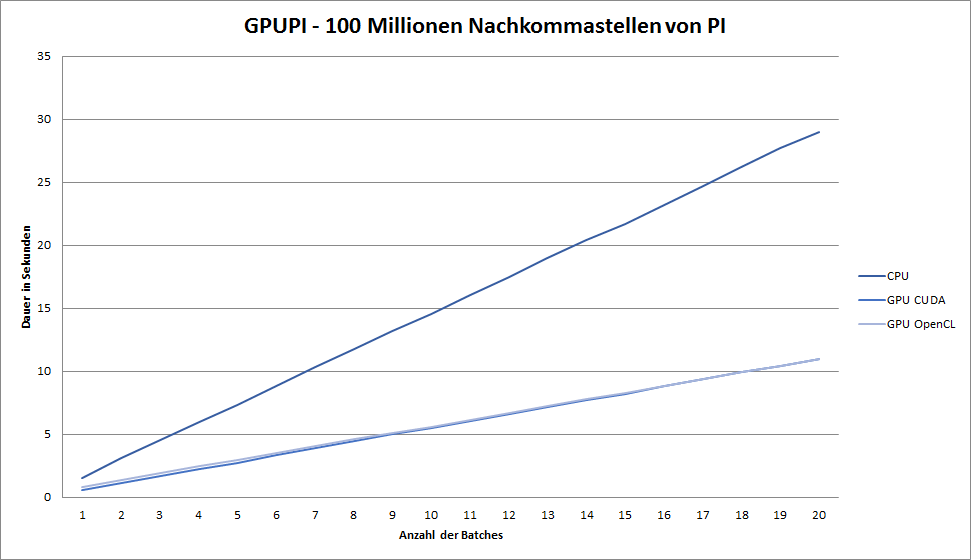
\includegraphics[width=1.0\linewidth]{images/GPUPI_100M.png}
		\caption{GPUPI 100 Millionen Nachkommastellen}
		\label{GPUPI_100M}
	\end{center}
\end{figure}

\begin{figure}[!h]
	\begin{center}
		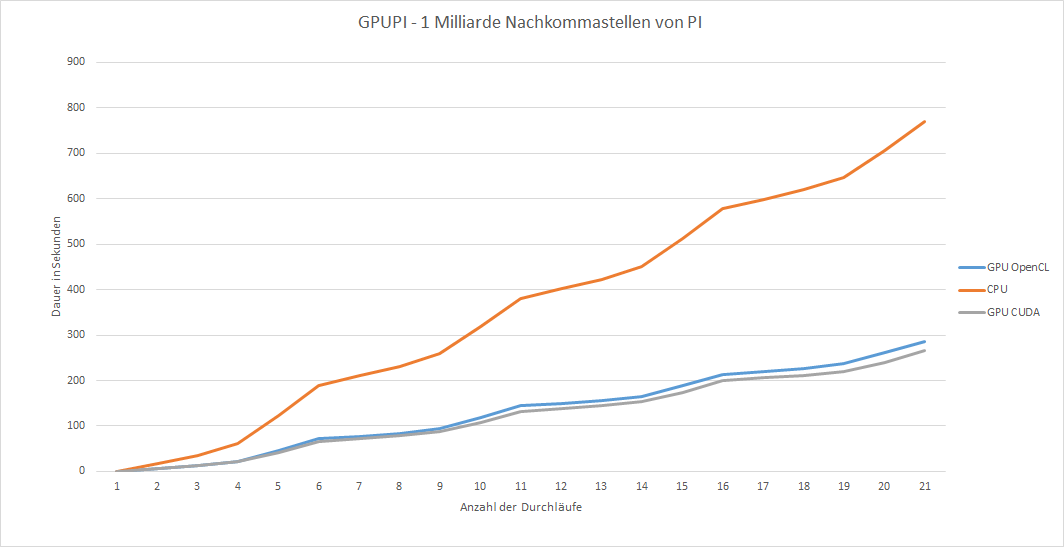
\includegraphics[width=1.0\linewidth]{images/GPUPI_1B.png}
		\caption{GPUPI 1 Milliarde Nachkommastellen}
		\label{GPUPI_1B}
	\end{center}
\end{figure}

\begin{figure}[!h]
	\begin{center}
		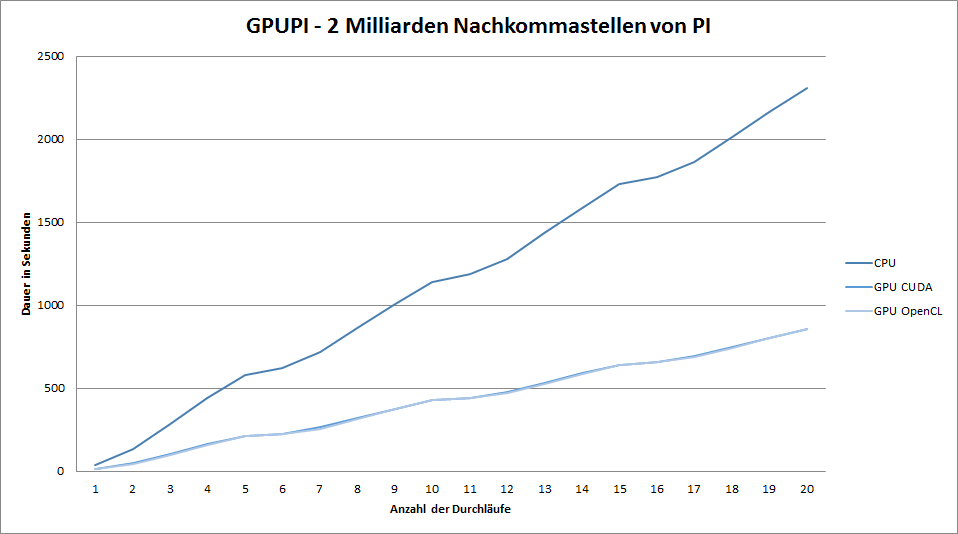
\includegraphics[width=1.0\linewidth]{images/GPUPI_2B.png}
		\caption{GPUPI 2 Milliarden Nachkommastellen}
		\label{GPUPI_2B}
	\end{center}
\end{figure}

\begin{figure}[!h]
	\begin{center}
		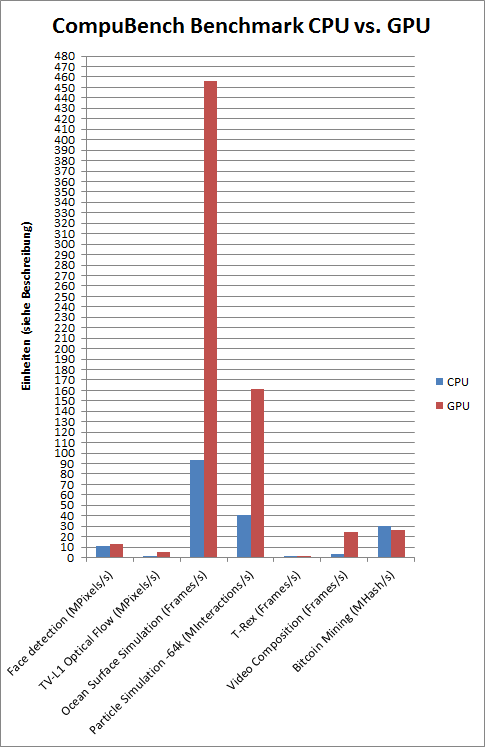
\includegraphics[width=0.8\linewidth]{images/CompuBench.png}
		\caption{Ergebnisse des CompuBench Benchmarks}
		\label{CompuBench}
	\end{center}
\end{figure}
\pagebreak
\subsubsection{Interpretation}
Es ist offensichtlich, dass die GPU bei deisem Anwendungsfall ihre Vorteile mit sich bringt. Sie liefert wesentlich schneller Ergebnisse, besonders bei der Berechnung von 2Milliarden Nachkommastellen Pi's ist der Unterschied der Rechenzeit zwischen GPU und CPU beträchtlich. Während man auf der CPU für die Berechnung 2308s (38min 28.217s) benötigt, braucht die GPU 856.5 (14min 16.559s) und hierbei handelt es sich letztlich nur um ein Beispiel mit eher geringem Umfang.\\
Der Unterschied zwischen CUDA und OpenCL wird nicht zu deutlich, wobei bei kürzeren Berechnungen der Unterschied interessanterweise größer ausfällt als bei längeren.
